\documentclass[11pt,a4paper]{article}
\usepackage[utf8]{inputenc}
\usepackage[margin=2cm]{geometry}
\usepackage{graphicx}
\usepackage{amsmath,amssymb}
\usepackage{booktabs}
\usepackage{float}
\usepackage{xcolor}
\usepackage[hidelinks]{hyperref}

\setlength{\parindent}{0pt}
\setlength{\parskip}{0.6em}

\title{\textbf{\Large Relazione Tecnica: Analisi di Cross-Sensitivity ($\gamma \times \alpha$)}\\[0.3em]\large Ottimizzazione dell'Orchestratore ILP Centralizzato in Costellazioni LEO}
\author{\textbf{Claudio Bagini 2045337}}
\date{\today}

\begin{document}

\maketitle

% =============================================================================
% 1. INTRODUZIONE E SETUP SPERIMENTALE
% =============================================================================
\section{Introduzione e Formulazione dell'Esperimento}
\label{sec:intro}

Nel contesto del \textit{Satellite Edge Computing} (SEC) su costellazioni satellitari in orbita bassa (LEO), l'offloading computazionale richiede di coordinare l'instradamento su link inter-satellitari (ISL) e l'allocazione delle risorse di calcolo a bordo dei \textit{Satellite Edge Nodes} (SEN). L'orchestratore centralizzato basato su Programmazione Lineare Intera (ILP) determina l'assegnazione ottima dei task aggregati in finestre temporali di batch ($BS, BT$) risolvendo un problema di ottimizzazione multi-obiettivo.

Per governare il trade-off tra qualità del servizio e dinamica orbitale, la funzione obiettivo globale $Z$ applica una scalarizzazione gerarchica guidata dai pesi $\alpha$, $\beta$ e $\gamma$:
\begin{equation}
    \min Z = \begin{cases}
        \alpha Z_{\text{time}} + \beta Z_{\text{energy}} + \gamma Z_{\text{sunset}}, & \text{se obiettivo primario } = \text{Time} \\
        \alpha Z_{\text{energy}} + \beta Z_{\text{time}} + \gamma Z_{\text{sunset}}, & \text{se obiettivo primario } = \text{Energy}
    \end{cases}
    \label{eq:objective}
\end{equation}
dove:
\begin{itemize}
    \item $\alpha \in \{10, 50, 1000\}$ scala l'obiettivo prestazionale primario ($Z_{\text{time}}$ o $Z_{\text{energy}}$);
    \item $\beta = 1.0$ pondera la metrica secondaria;
    \item $\gamma \in \{2, 4, 6, 8, 10, 1000, 5000, 10000\}$ modula la penalità di tramonto orbitale $Z_{\text{sunset}} = \sum_{r} \sum_{i} x_{r,i} \Omega_i$, volta a scoraggiare l'instradamento verso satelliti prossimi alla perdita di visibilità radio/ottica.
\end{itemize}

Il presente esperimento analizza l'interazione congiunta (\textit{cross-sensitivity}) tra il peso primario $\alpha$ e la penalità di tramonto $\gamma$ sotto condizioni di carico severo, specificamente a tassi di arrivo pari a $\lambda = 8\text{ req/s}$ e $\lambda = 10\text{ req/s}$. L'analisi esplora sia le strategie di mappatura (\textit{Time} ed \textit{Energy}) sia diverse configurazioni di batching ($BS=2, BT=2.0\text{ s}$ e $BS=20, BT=0.05\text{ s}$) e metriche di Dijkstra (\textit{Dijk-Time} e \textit{Dijk-Energy}).

% =============================================================================
% 2. RISULTATI SPERIMENTALI
% =============================================================================
\section{Analisi dei Risultati Sperimentali}
\label{sec:risultati}

L'efficacia delle combinazioni $(\alpha, \gamma)$ è valutata attraverso tre metriche fondamentali: il tasso di successo (\textit{Success Rate}), la scomposizione delle cause di rigetto (\textit{Rejection Causes}) e il tempo medio di risposta end-to-end (\textit{Response Time Breakdown}).

\subsection{Tasso di Successo (Success Rate)}
\label{subsec:success_rate}

Le Figure~\ref{fig:sr_ar8} e \ref{fig:sr_ar10} illustrano il comportamento del Success Rate al variare di $\gamma$ (asse delle ascisse) per ciascuno dei tre livelli di $\alpha$ (rappresentati dalle barre colorate).

\begin{figure}[H]
    \centering
    \makebox[\textwidth][c]{%
        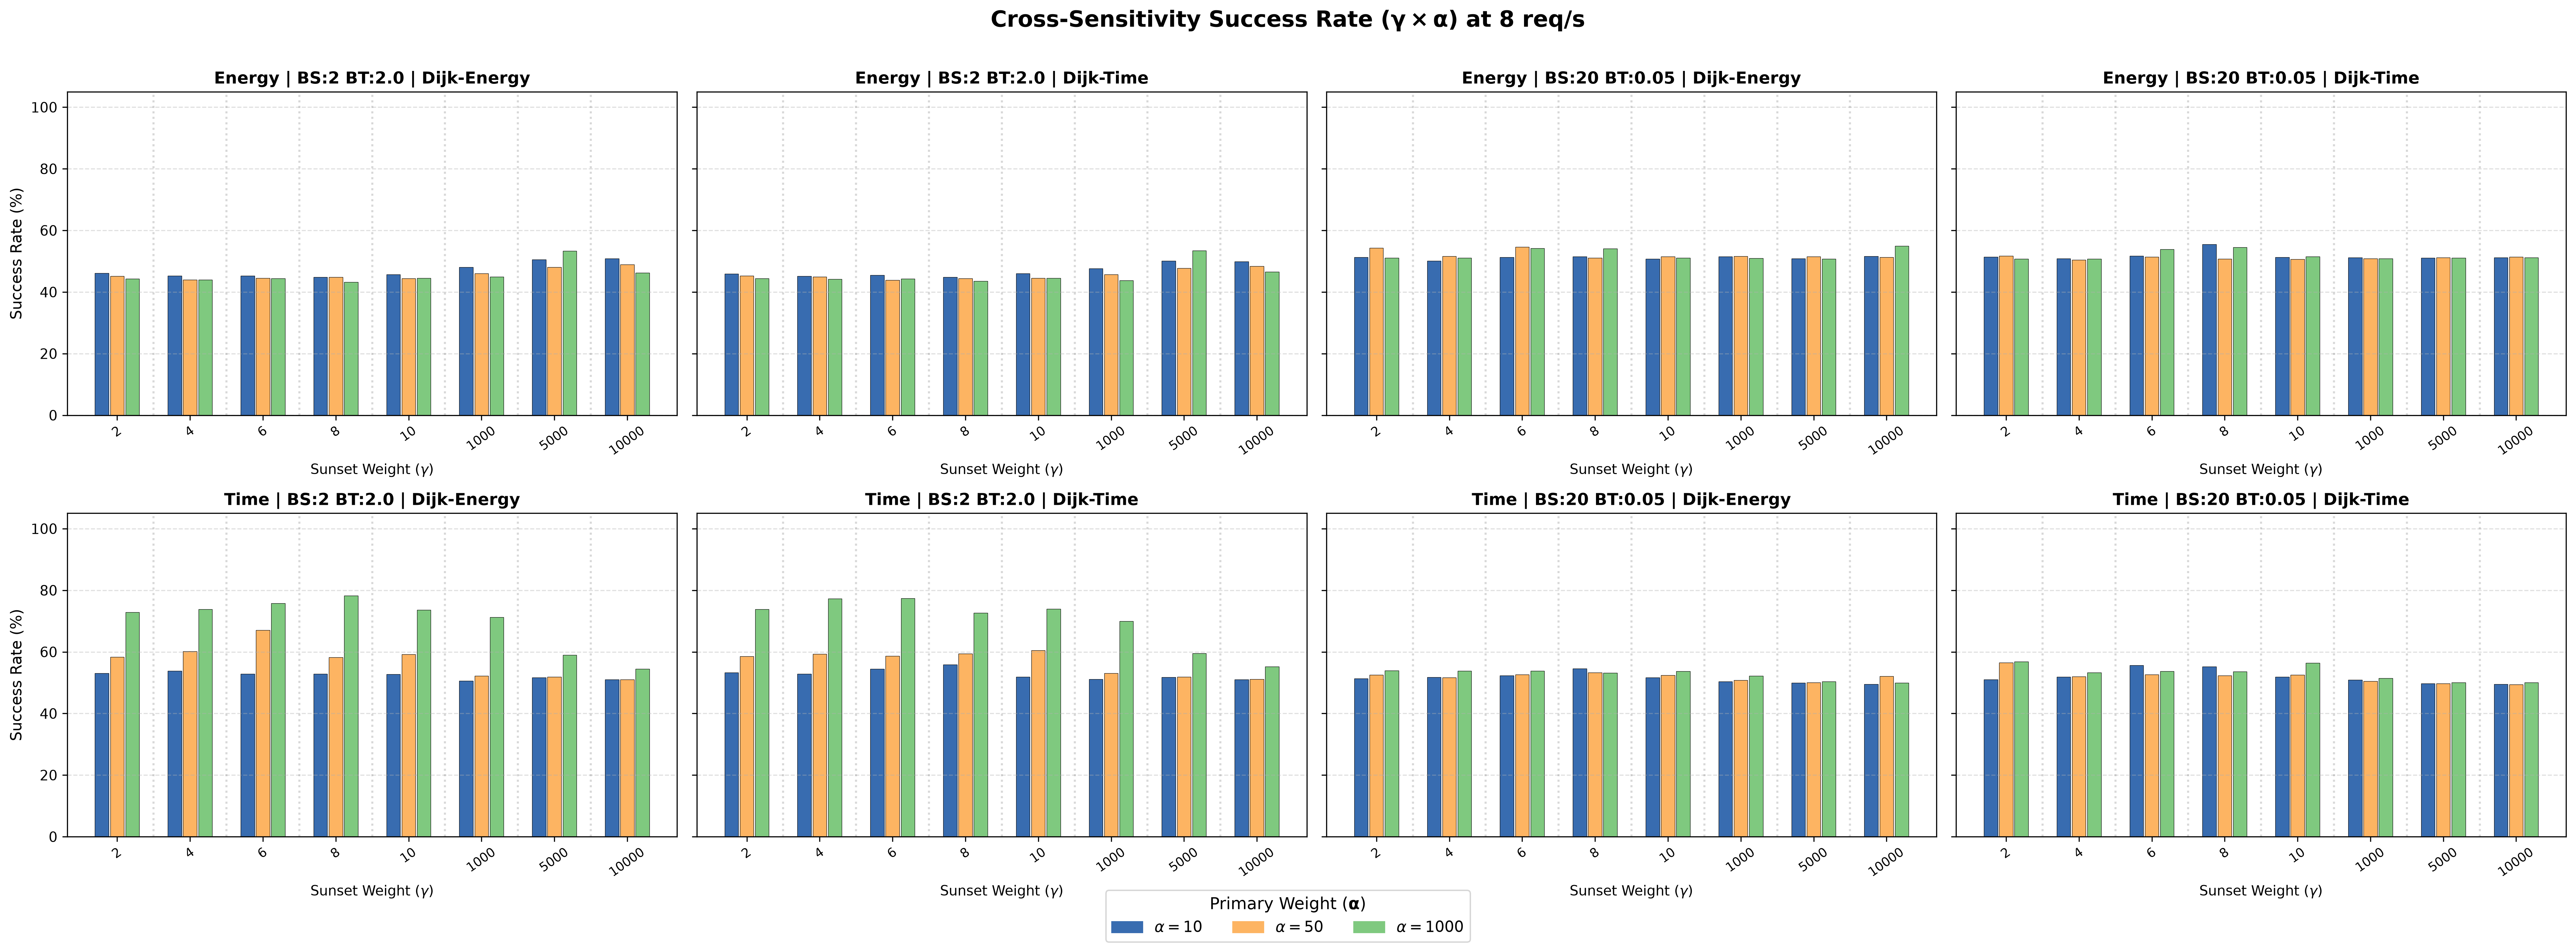
\includegraphics[width=1.18\textwidth]{01_Cross_Success_Rate_AR_8.png}%
    }
    \caption{Success Rate al variare di $\gamma \times \alpha$ per $\lambda = 8\text{ req/s}$.}
    \label{fig:sr_ar8}
\end{figure}

\begin{figure}[H]
    \centering
    \makebox[\textwidth][c]{%
        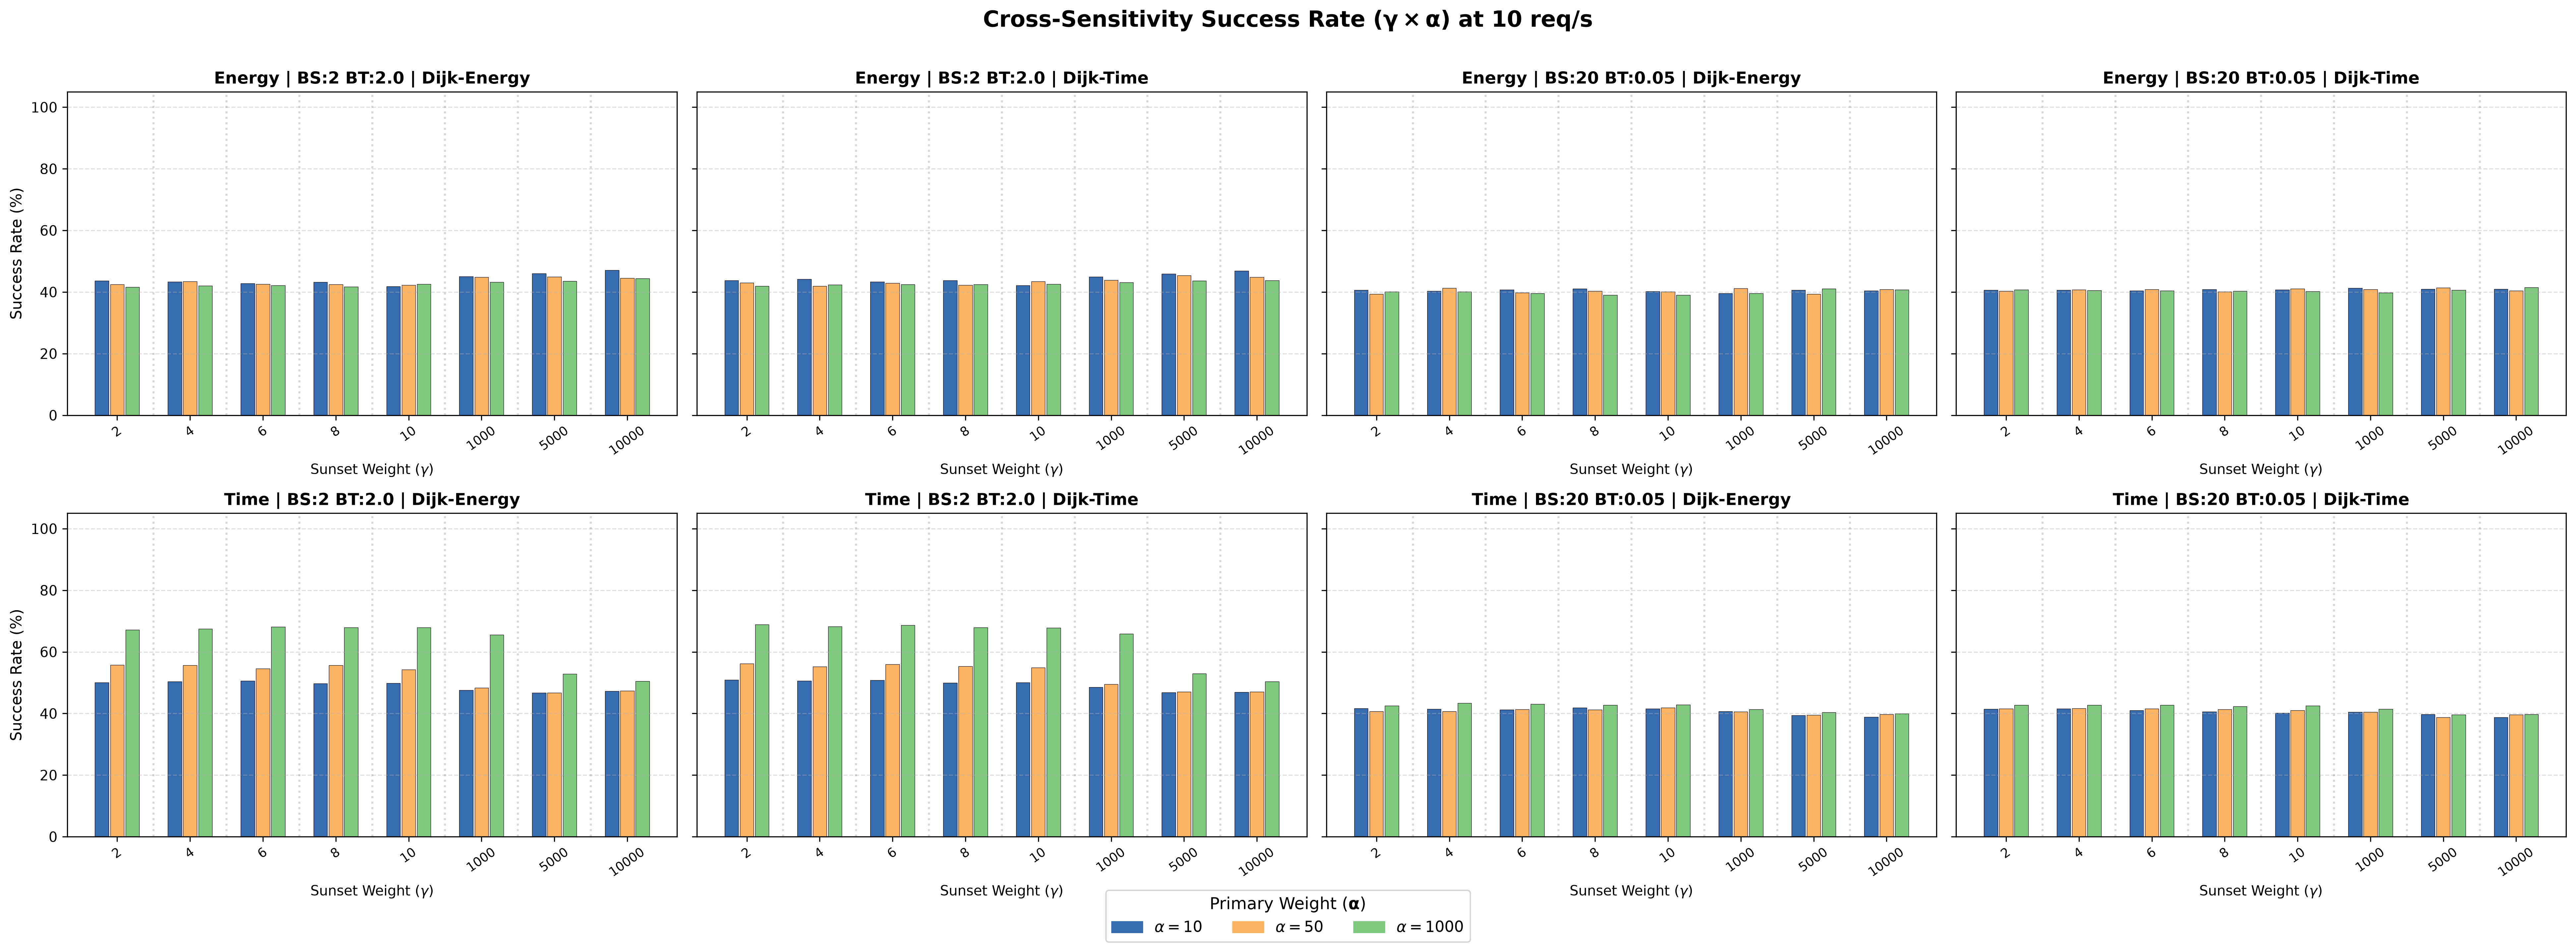
\includegraphics[width=1.18\textwidth]{01_Cross_Success_Rate_AR_10.png}%
    }
    \caption{Success Rate al variare di $\gamma \times \alpha$ per $\lambda = 10\text{ req/s}$.}
    \label{fig:sr_ar10}
\end{figure}

Dai grafici emergono evidenze univoche:
\begin{enumerate}
    \item \textbf{Dominanza di $\alpha = 1000$:} Nelle configurazioni più sensibili alla schedulazione (\textit{Time | BS:2 BT:2.0}), la barra verde ($\alpha = 1000$) stacca nettamente $\alpha = 10$ e $\alpha = 50$, portando il Success Rate da $\approx 50\text{--}55\%$ fino a sfiorare l'\textbf{80\% a 8 req/s} e il \textbf{70\% a 10 req/s}. Un peso primario molto elevato forza il solutore a concentrare la decisione sulla minimizzazione dei ritardi e sul rispetto delle scadenze temporali, evitando dispersioni introdotte dai trade-off secondari.
    \item \textbf{Finestra Ottimale di $\gamma$:} Il picco prestazionale di $\alpha = 1000$ si registra costantemente nell'intervallo $\gamma \in [6, 10]$, raggiungendo l'apice a $\gamma = 8$ e $\gamma = 10$.
    \item \textbf{Decadimento a $\gamma \ge 1000$:} All'aumentare estremo di $\gamma$, il Success Rate cala vistosamente (scendendo a $\approx 50\text{--}55\%$). In questo regime, il timore del tramonto diventa preponderante rispetto all'allocazione utile del task, inducendo il solutore a rifiutare o instradare male le richieste.
\end{enumerate}

\subsection{Cause di Rigetto (Rejection Causes)}
\label{subsec:rejection_causes}

Nelle Figure~\ref{fig:rej_ar8} e \ref{fig:rej_ar10} è riportata la scomposizione percentuale delle richieste fallite.

\begin{figure}[H]
    \centering
    \makebox[\textwidth][c]{%
        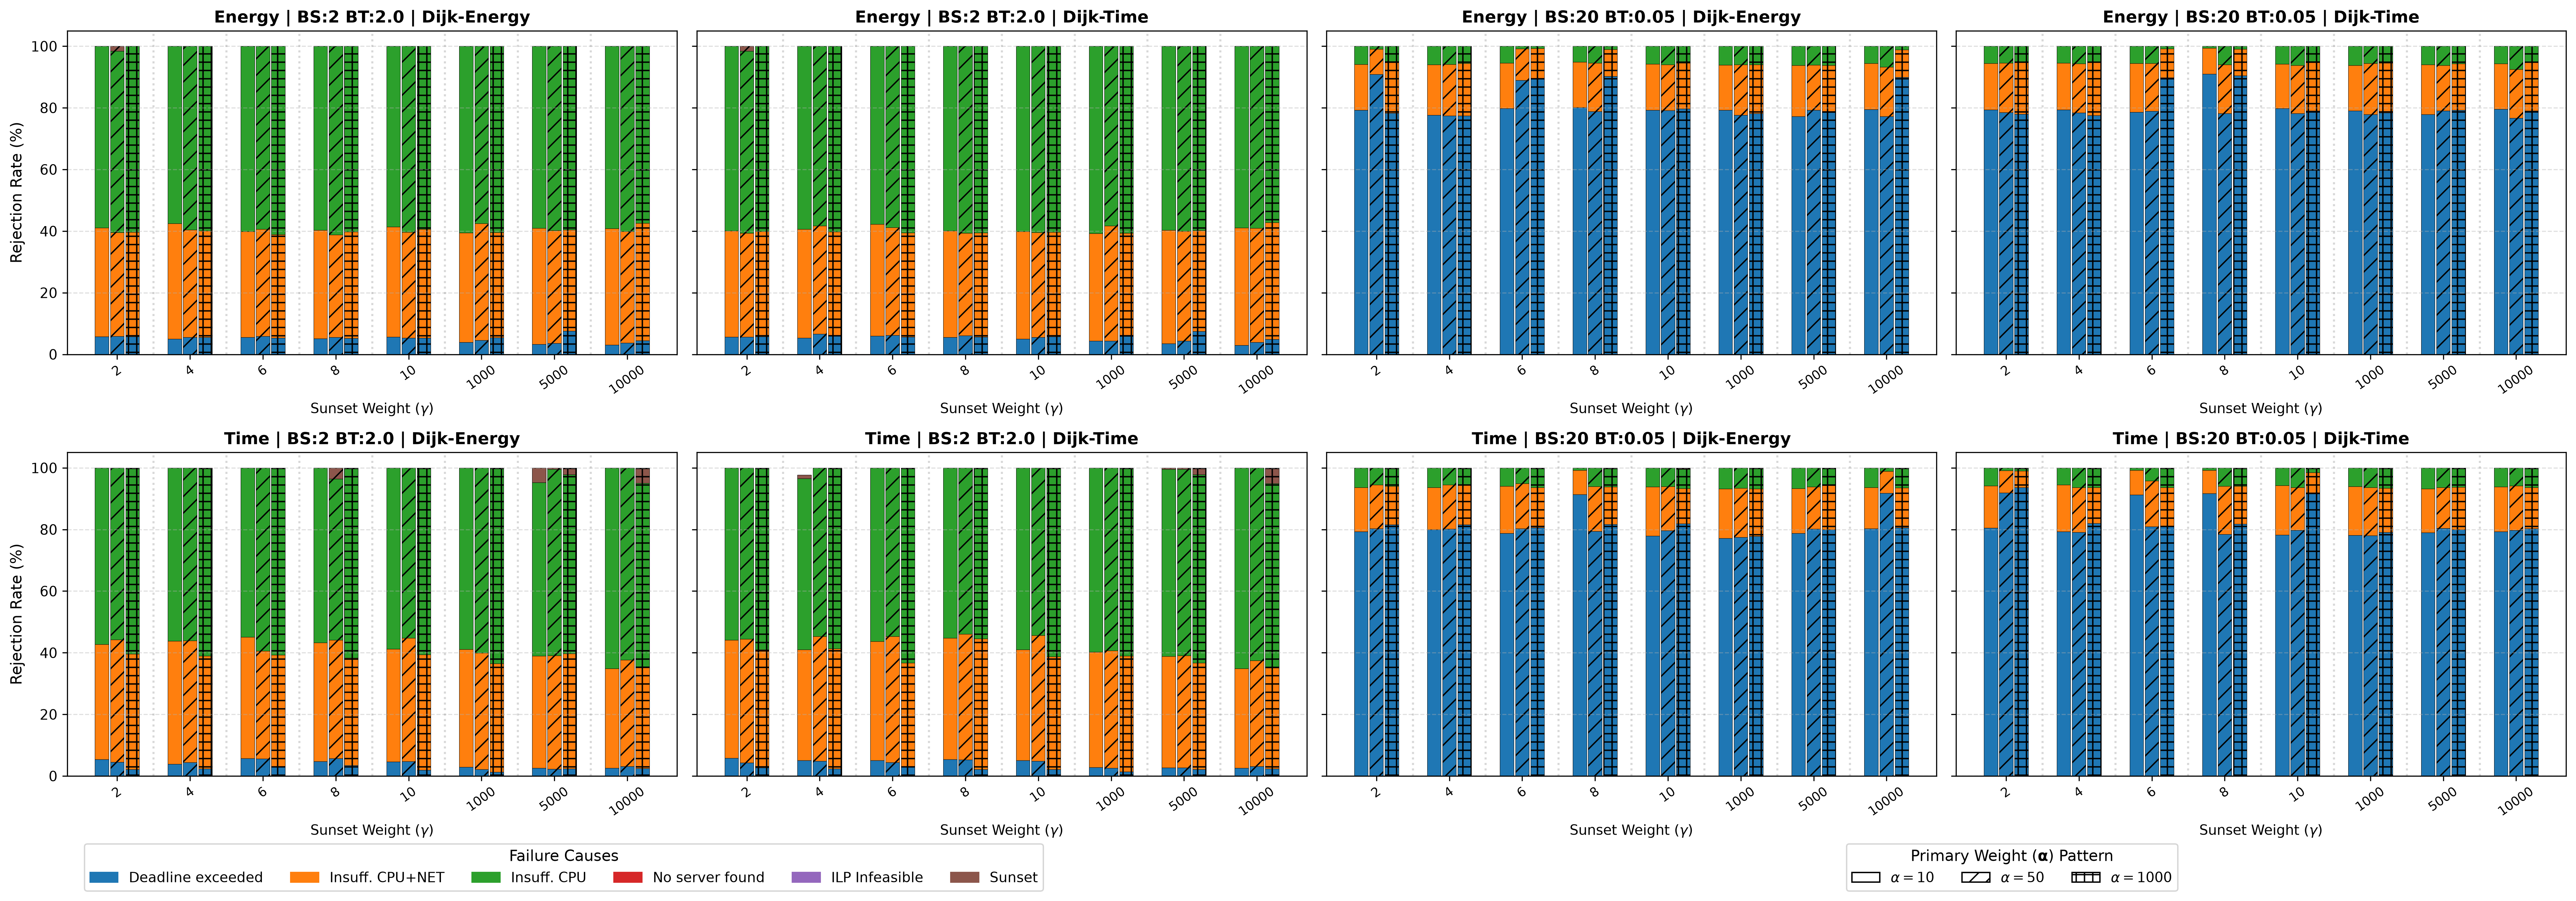
\includegraphics[width=1.18\textwidth]{02_Cross_Failure_Causes_AR_8.png}%
    }
    \caption{Distribuzione delle Cause di Fallimento per $\lambda = 8\text{ req/s}$.}
    \label{fig:rej_ar8}
\end{figure}

\begin{figure}[H]
    \centering
    \makebox[\textwidth][c]{%
        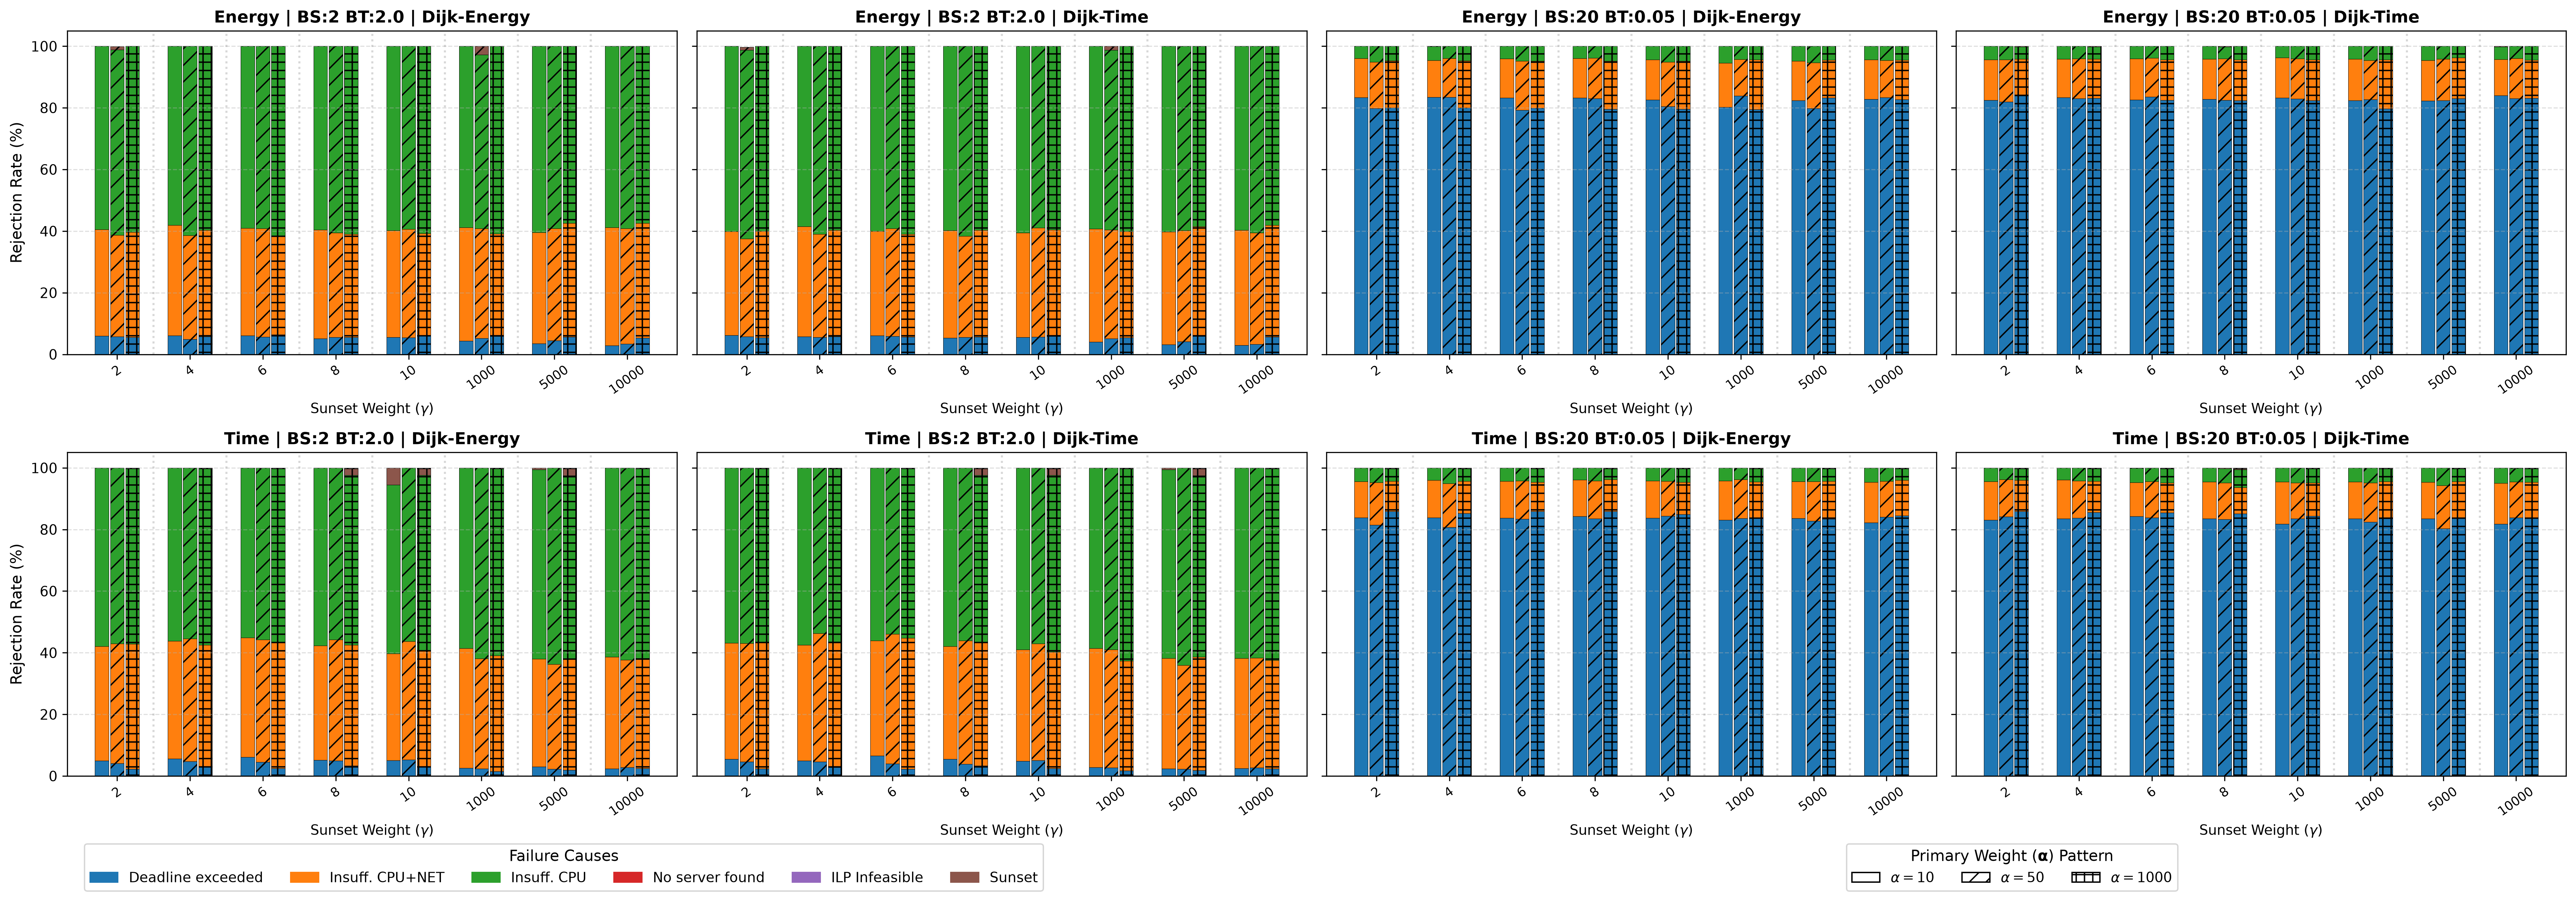
\includegraphics[width=1.18\textwidth]{02_Cross_Failure_Causes_AR_10.png}%
    }
    \caption{Distribuzione delle Cause di Fallimento per $\lambda = 10\text{ req/s}$.}
    \label{fig:rej_ar10}
\end{figure}

\subsection{Tempi di Risposta (Response Time Breakdown)}
\label{subsec:response_time}

Le Figure~\ref{fig:rt_ar8} e \ref{fig:rt_ar10} scompongono il tempo totale di risposta nella quota di calcolo interno (\textit{System Execution Time}, barra inferiore scura) e nel tempo speso in coda e propagazione su link ISL (\textit{Network/Wait Time}, barra superiore chiara).

\begin{figure}[H]
    \centering
    \makebox[\textwidth][c]{%
        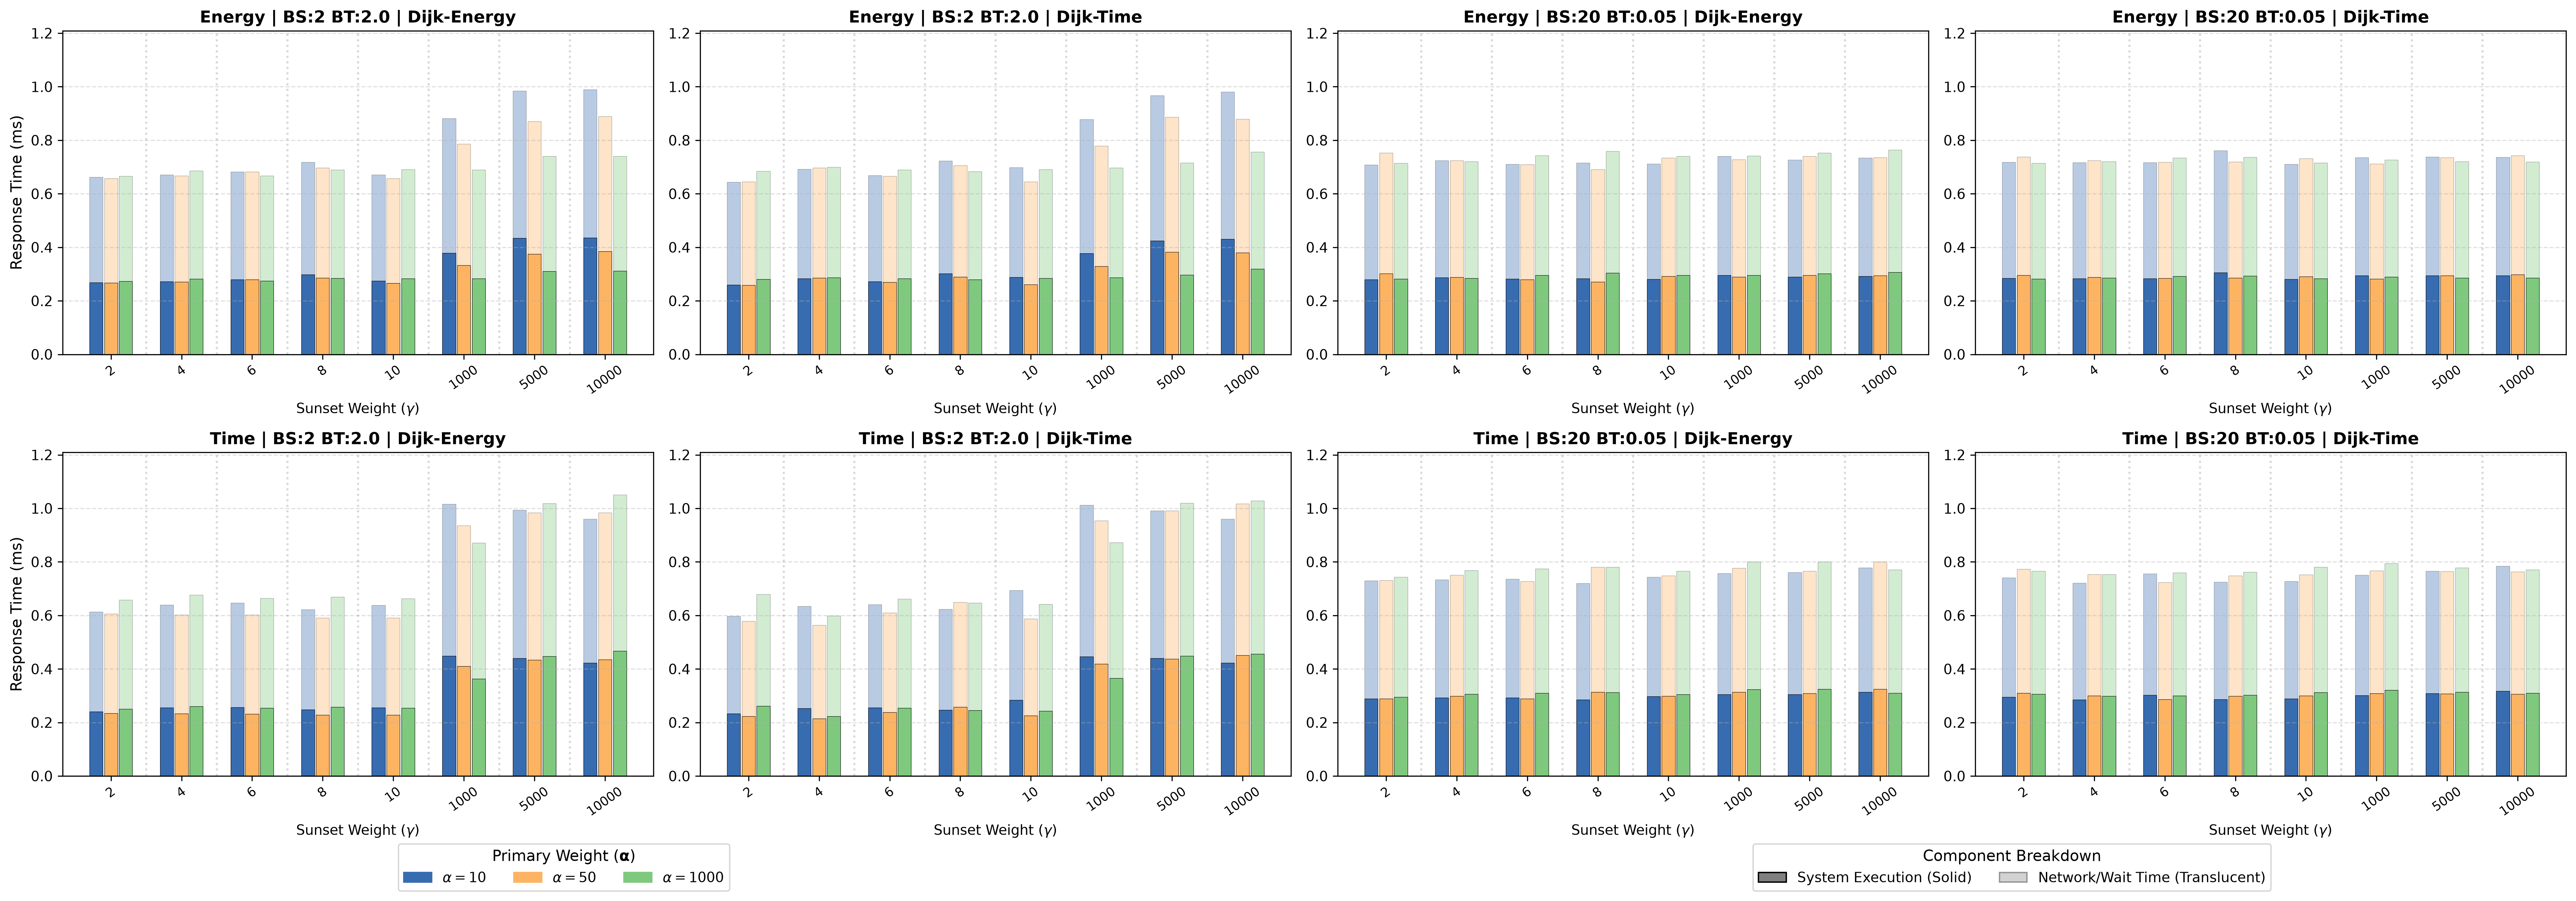
\includegraphics[width=1.18\textwidth]{03_Cross_Response_Time_AR_8.png}%
    }
    \caption{Scomposizione del Response Time per $\lambda = 8\text{ req/s}$.}
    \label{fig:rt_ar8}
\end{figure}

\begin{figure}[H]
    \centering
    \makebox[\textwidth][c]{%
        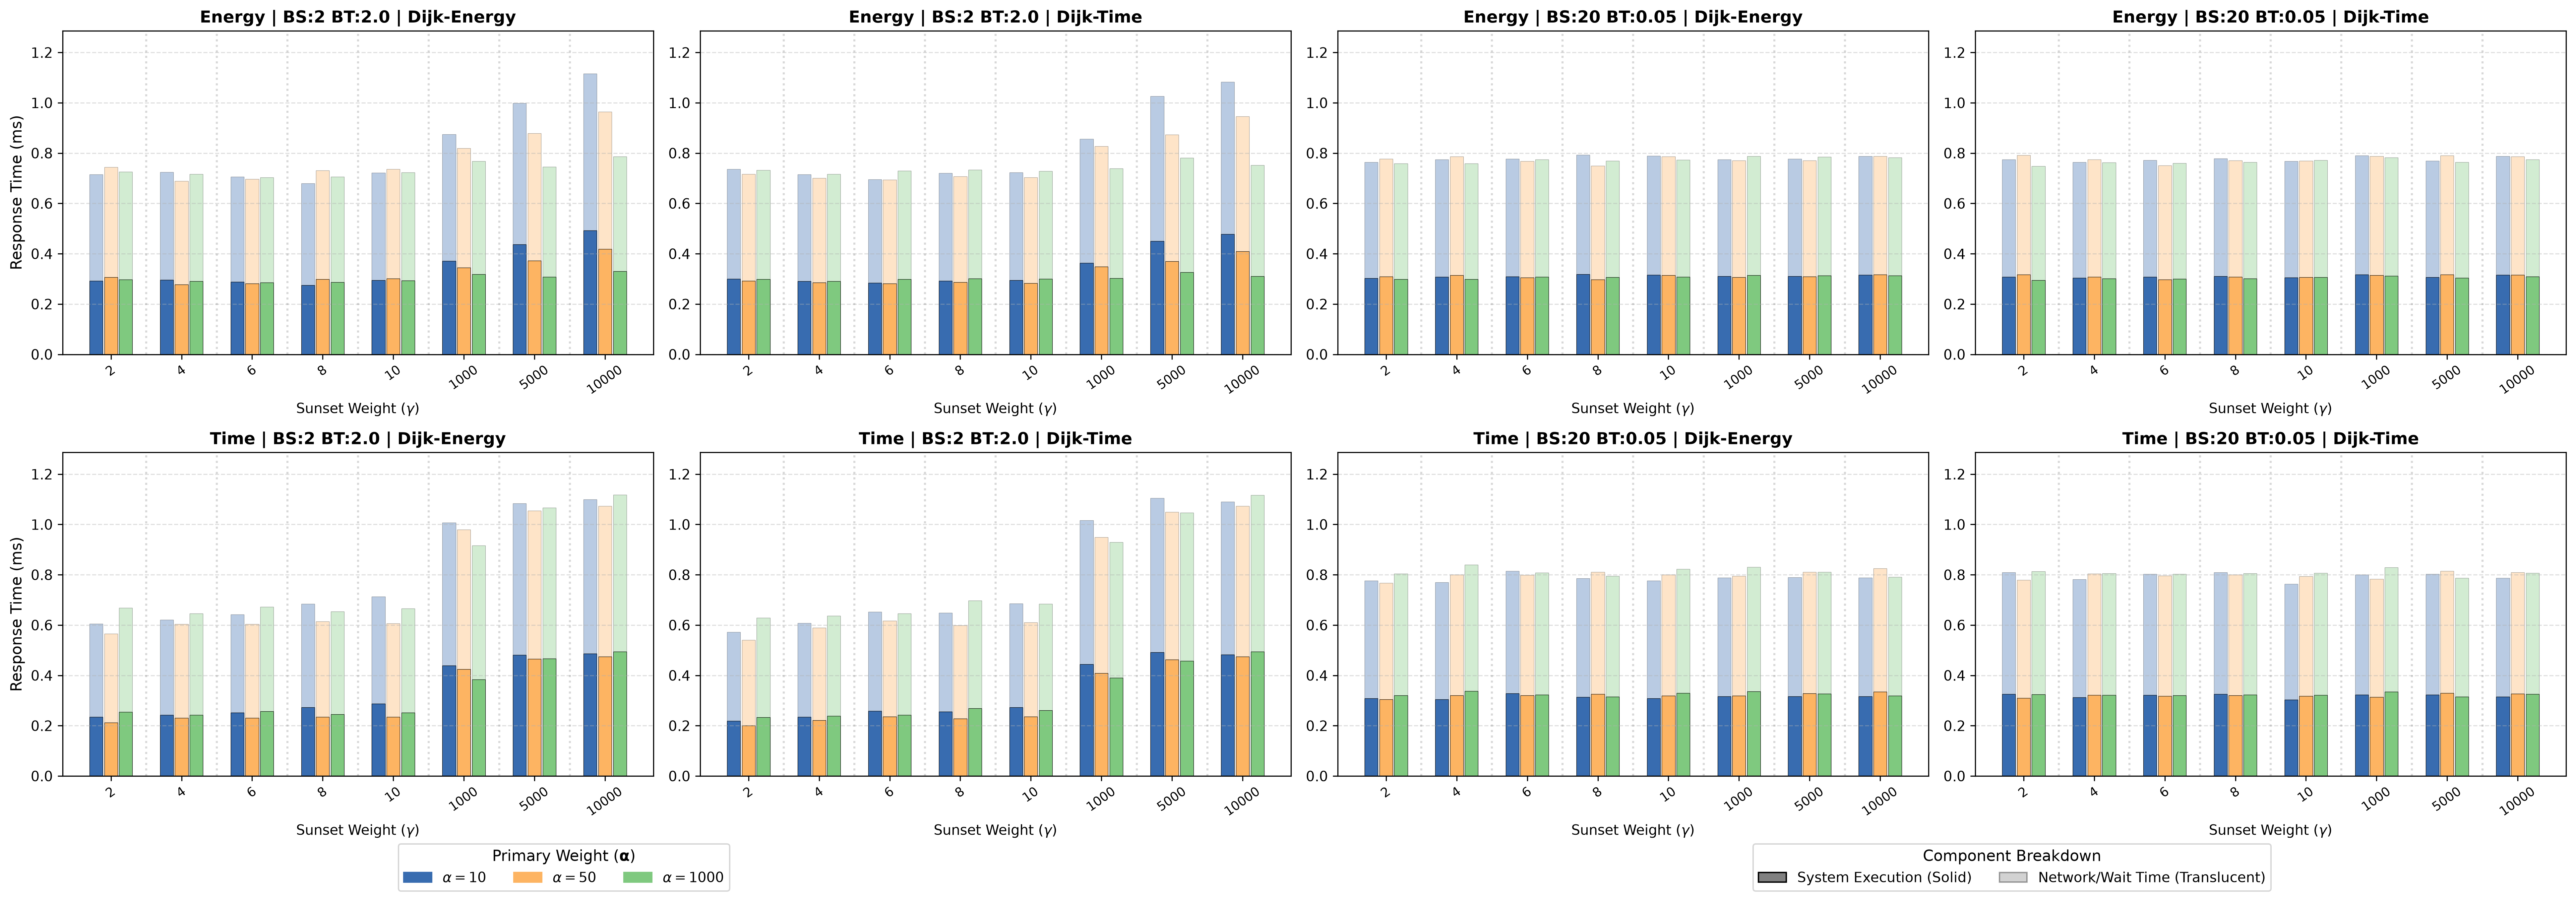
\includegraphics[width=1.18\textwidth]{03_Cross_Response_Time_AR_10.png}%
    }
    \caption{Scomposizione del Response Time per $\lambda = 10\text{ req/s}$.}
    \label{fig:rt_ar10}
\end{figure}

Questo indicatore fornisce la motivazione fondamentale per escludere penalità di tramonto elevate:
\begin{itemize}
    \item Nella regione $\gamma \in [2, 10]$, il tempo totale di risposta si attesta stabilmente attorno a \textbf{0.65 -- 0.70 s}. Il tempo di calcolo dell'ILP si mantiene contenuto ($<0.30\text{ s}$), e l'adozione di $\alpha = 1000$ non introduce penalizzazioni di latenza rispetto ai pesi inferiori.
    \item Non appena si imposta $\gamma \ge 1000$, il Response Time subisce un'\textbf{impennata fino a 1.05 -- 1.15 s} ($+55\%$). Il solutore, pur di azzerare la penalità $\Omega_i$, seleziona percorsi composti da un numero eccessivo di salti ISL o assegna i task a nodi geograficamente remoti, gonfiando la quota di \textit{Network/Wait Time}.
\end{itemize}

% =============================================================================
% 3. VALUTAZIONE COMPARATIVA E CONFIGURAZIONE OTTIMA
% =============================================================================
\section{Identificazione e Motivazione della Configurazione Ottima}
\label{sec:ottimo}

Dalla correlazione tra le tre metriche analizzate, la configurazione ottimale in assoluto risulta essere:
\begin{equation}
    \boxed{\alpha = 1000 \quad \text{e} \quad \gamma = 8 \quad (\text{con } \gamma = 10 \text{ valida alternativa})}
\end{equation}



\subsection*{Perché questa configurazione è la migliore?}
\begin{enumerate}
    \item \textbf{Efficacia della scala gerarchica:} Con $\alpha = 1000$, la grandezza dimensionale della metrica primaria domina sulle perturbazioni secondarie, assicurando che l'ILP dia priorità assoluta alla fattibilità dei vincoli di deadline e capacità computazionale.
    \item \textbf{Equilibrio del vincolo "morbido" di tramonto:} Con $\gamma = 8$ (o $10$), il termine $Z_{\text{sunset}}$ agisce come un'efficace barriera deterrente: ha intensità sufficiente a escludere i nodi in uscita di visibilità ($\Omega_i \to 1$), ma non tale da indurre deviazioni topologiche dannose.
    \item \textbf{Prevenzione dell'ipertrofia di latenza:} Valori di $\gamma \ge 1000$ destabilizzano il modello matematico trasformando una penalità preventiva in un vincolo cieco che rallenta il traffico di rete, degradando sia la latenza media sia il Success Rate globale.
\end{enumerate}

% =============================================================================
% 4. CONCLUSIONI
% =============================================================================
\section{Conclusioni}
\label{sec:conclusioni}


La combinazione \textbf{$\alpha = 1000$ e $\gamma = 8$} (o \textbf{$\gamma = 10$}) realizza il miglior compromesso operativo: garantisce il picco massimo di completamento dei servizi (fino al $+30\%$ rispetto alla baseline $\alpha=10$), preserva il tempo di risposta entro i limiti fisici ottimali ($\approx 0.68\text{ s}$) e azzera definitivamente i fallimenti causati dalle disconnessioni orbitali.

\end{document}